\chapter{Results and Conclusions}\label{triumphantDataChapter}

The injection locking was successful and I successfully produced two working beams with an adjustable detuning. I have verified that both beams' frequencies are coupled to and offset from the master laser. Furthermore, the output from the slaves is sufficient to drive the transition. 

\section{Brief note on data from the spectrum analyzer}

The main way that we can see if the lasers are working properly is to couple them to the spectrum analyzer, which was discussed in Section\,\ref{spectAnalayzer} and Appendix\,\ref{SpectrumAnalyzerAppendix}. The spectrum analyzer is an optical cavity whose length is being changed as a function of time. A photo diode on the end of the spectrum analyzer captures a signal that is proportional to the transmission through the spectrum analyzer cavity. This signal is read on an oscilloscope.

For all of the data in this thesis, the length of the spectrum analyzer was modulated in a sawtooth pattern. Thus, the length of the cavity changed at a constant speed over some interval before being quickly brought back to its original length. A typical scan typically involves changing the length of the cavity by $\sim$3$\mu$m. 

%todo: put in a picture of the cavity

The output of the photo diode is sent to an oscilloscope that is triggered by the frequency generator that also modulates the piezoelectric actuators on the spectrum analyzer. Therefore, typical data from the spectrum analyzer is a trace from an oscilloscope. The $y$ axis represents signal from the photo diode, while the $x$ dimension represents time elapsed since the last triggering event. The $x$ axis values in the regimes shown in Figures\,\ref{fig:slaveMaster} and \ref{fig:typicaldata} are also proportional to the change in length of the cavity because the cavity length is changing linearly as a function of time during the parts of the scan that I am showing. Because each sweep of the sawtooth function generator and piezo driver is identical, we can safely compare subsequent traces to track the relative frequency changes of any given peak. 

If we scan about $\sim$2$\mu$m, we expect that the peaks corresponding to our 408 nm lasers will go in in and out of resonance $\sim$5 times. Therefore, we would expect that in the oscilloscope trace, the same peak should be repeated approximately five times. For this cavity, the free spectral range is 187 MHz. This means that the distance between two peaks from the the same spectral component of the light in our scan will correspond to the distance that any given peak would move by if it were detuned by 187 MHz. This gives us a natural scale by which to judge the movement of peaks. 

However, note that the detunings relevant to this experiment are on the order of GHz, which is much larger than the free spectral range of the cavity. This simply means that two nearby peaks coming from different lasers are from different modes of the spectrum analyzer. 

%fsr corresponds to different lengths for different lasers 

\section{Tracking slave lasers with master laser}

First, when we look at one slave and the master laser on the spectrum analyzer and scan the master laser, we see that the slave scans with the master laser. This is illustrated in Figure\,\ref{fig:slaveMaster}.

\begin{figure}
    %\centerline{\includegraphics[trim=100pt 100pt 100pt 100pt, clip=true, totalheight=0.5\textheight,angle=90]{testfigure}}
    %\centerline{\includegraphics[totalheight=0.3\textheight]{testfigure}}
    \centerline{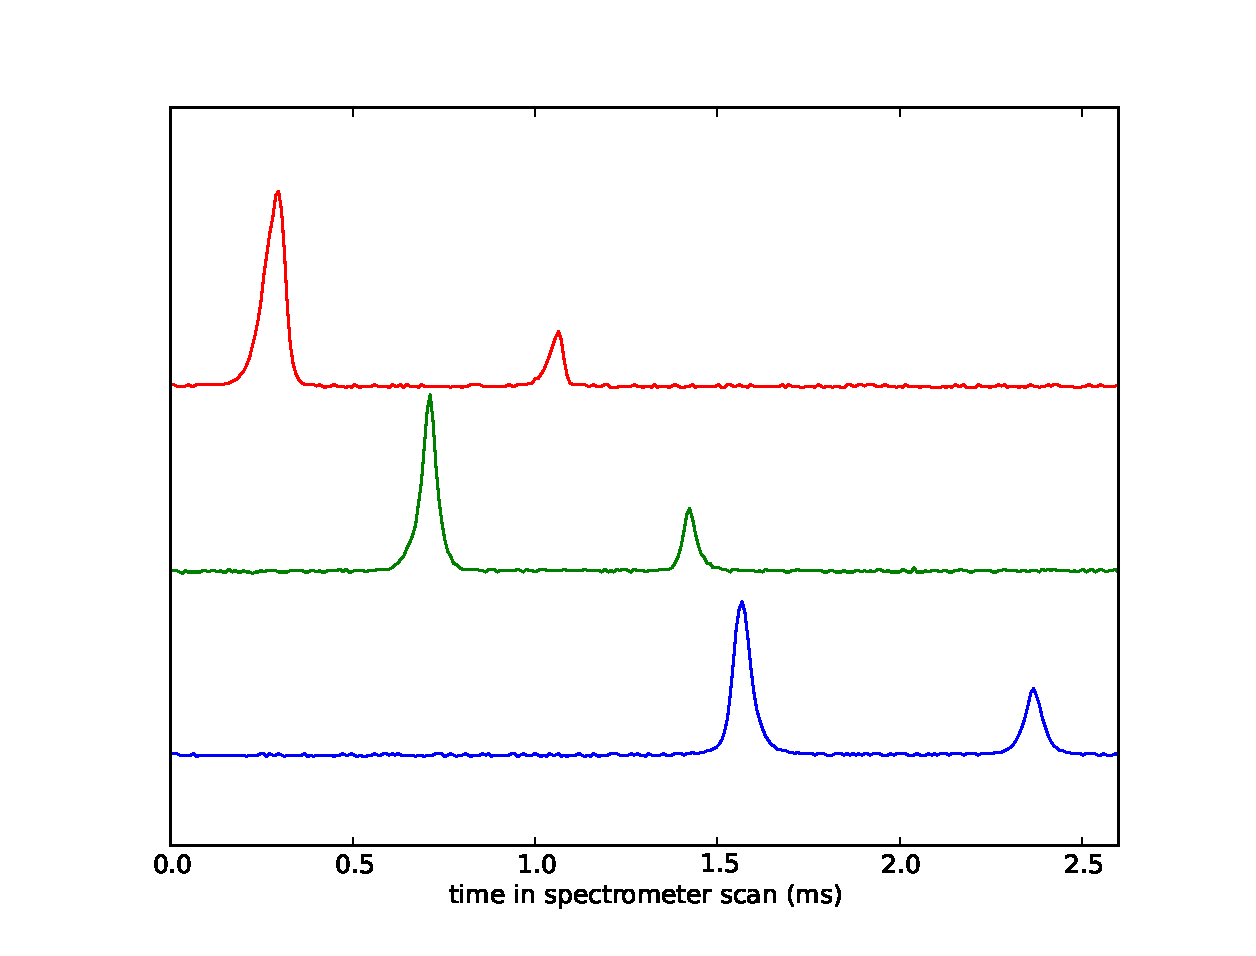
\includegraphics[width=0.9\textwidth]{Slave2AndMasterScanningMaster}}
    %\includegraphics[totalheight=0.3\textheight]{testfigure}
    \caption[Slave laser and master laser frequencies tracking together]{\label{fig:slaveMaster}
    The slave and master laser on the spectrum analyzer. The y axis is the signal on the spectrum analyzer. There are three traces here, each showing the master laser at a different frequency. The slave laser is the taller peak, while the other peak belongs to the master laser. The peaks corresponding to the master laser and the slave laser move together. Each trace is offset in the $y$ direction in order to make it visible.}
\end{figure}

\section{Verifying that the slave frequencies can be adjusted with the RF oscillator}
Second, I examined the output of the spectrum analyzer while both slave lasers were coupled into it. 
The two peaks clearly corresponded to the two slave lasers, which we verified by alternatively blocking each of the slaves. 

%We can see that there is a lot of power 

I performed an experiment where I adjusted the driving frequency of the rf frequency generator that drives the AOM. I observed that the peaks on the spectrum analyzer shifted by an amount corresponding to the change in the frequency of the rf oscillator. This provides strong evidence that the two slaves were, indeed, injection locked to the modulated beams coming out of the AOM. This data is presented in Figure\,\ref{fig:typicaldata}.


%where is the energy going? I think it goes from reflecting to transmitting
%I'm curious about finding the contribution to the line width of the cavity from the peaks.
 
\begin{figure}
    %\centerline{\includegraphics[trim=100pt 100pt 100pt 100pt, clip=true, totalheight=0.5\textheight,angle=90]{testfigure}}
    %\centerline{\includegraphics[totalheight=0.3\textheight]{testfigure}}
    \centerline{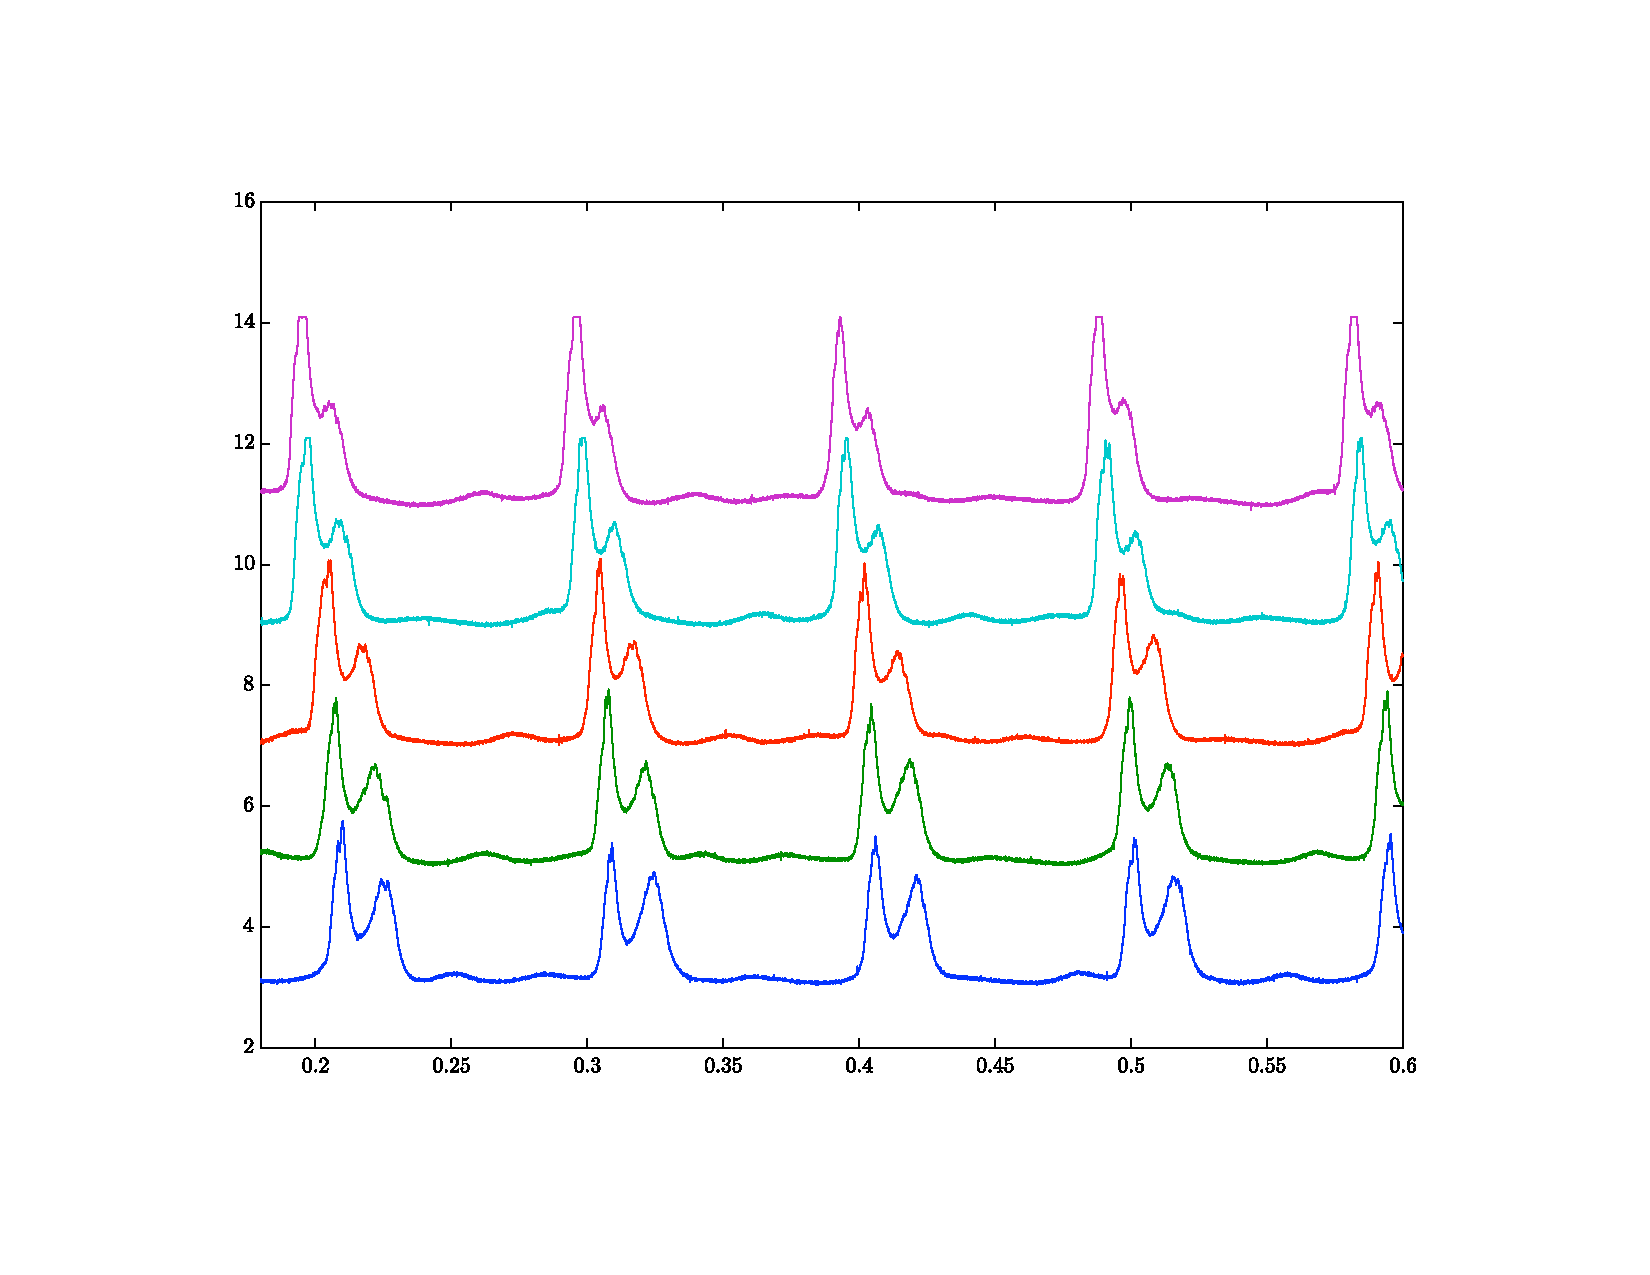
\includegraphics[width=0.9\textwidth]{sampleOffsetData}}
    %\includegraphics[totalheight=0.3\textheight]{testfigure}
    \caption[Scans of slave lasers for several rf oscillator frequencies]{\label{fig:typicaldata}
Scans of slave lasers for several rf oscillator frequencies. I changed the detuning on the frequency generator in 10 MHz increments between capturing each of these traces. The $y$ axis represents transmission through the spectrum analyzer cavity as measured by the photo diode and is presented in arbitrary units with the traces offset to enhance visibility. The $x$ axis represents time during the cavity scan. As the detuning changes, the distance between the two peaks shifts, thereby proving that the detuning between the slave laser and the master laser is controlled by the AOM and rf frequency generator.}
\end{figure}

%\begin{figure}
%\centerline{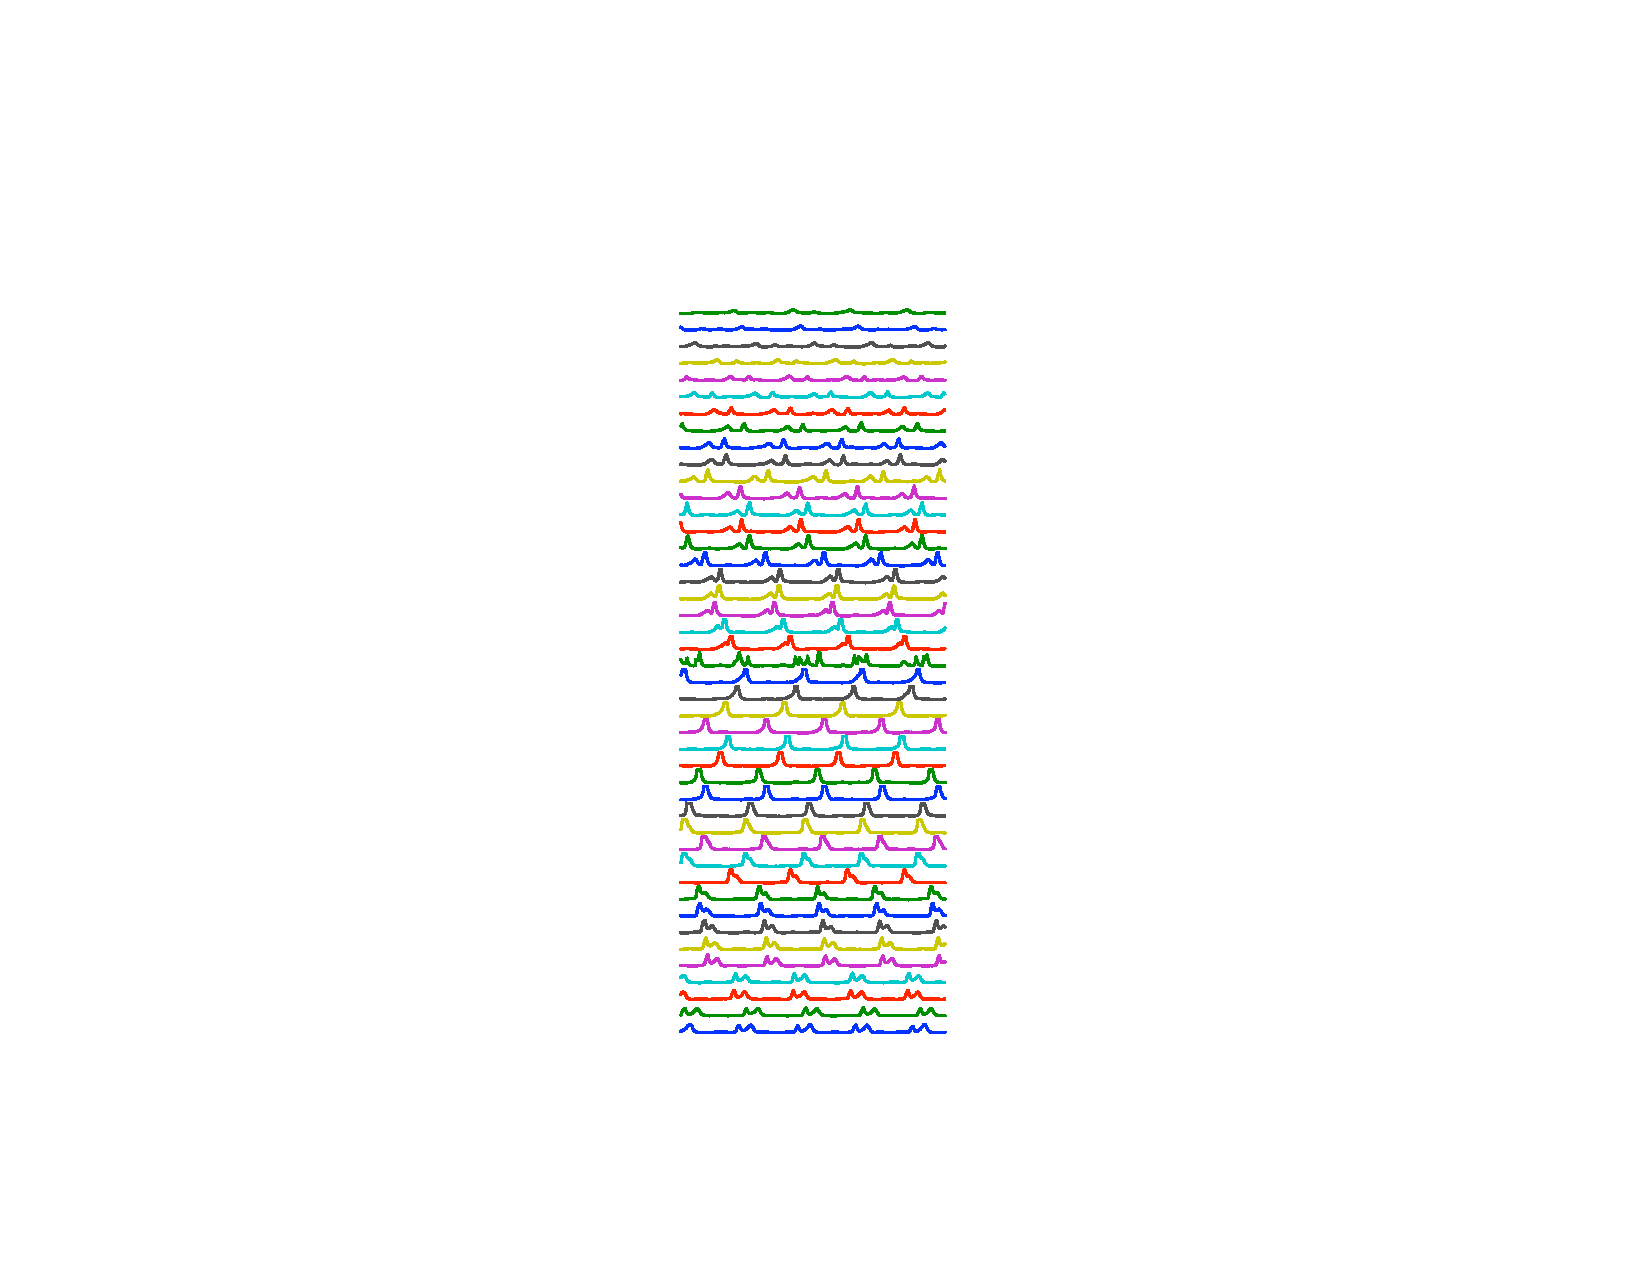
\includegraphics{all_splittingData}}
%\caption[Additional ]{\label{fig:alldata} 
%Spectrum analyzer data for }
%\end{figure}

%Also, I have data that I can analyze to examine the feasibility of a Chu lock. I recorded 999 traces that showed the output of the spectrum analyzer, the current and the voltage. I recorded these over several hours, during which the laser drifted into and out of good, single mode operation. In principle, this data could be analyzed. 

We have shown that we can change the rf oscillator frequency and thereby change the detuning. There are two limiting factors on the extent that we can do this. (Notice in Fig.\ \ref{fig:typicaldata} that the peaks get small as we continue to detune.) Both factors are geometrical in nature: First, the AOM diffraction efficiency decreases because the Bragg angle changes. Second, the diffraction angle changes, leading to a misalignment of the injected beams and a weakening of injection. However, even for large detunings, the injection lock can be achieved simply by realigning the output beams. We demonstrated this by successfully tuning the AOM driving frequency to the point where injection was lost, realigning (using the lasers as photo diodes) and then re-achieving successful injection lock.

\section{Summary and future work}
To summarize: I have built a laser system capable of driving stimulated Raman transitions between the $F=4$ and $F=5$ hyperfine levels of $^{87}$Sr$^+$. I successfully tuned and stabilized the master laser. Using an AOM, I generated two shifted beams that I used to injection lock two other lasers (slave 1 and slave 2).
%linewdith?

In order to ensure that the 408 nm 5 GHz detuned laser system works, we will need to actually drive stimulated Raman transitions in $^{87}$Sr$^+$. Completion of this requires the completion of the LVIS and other parts of the experiment. Getting the transition rate right will also likely require tweaks to many of the parameters of the current system. There are also additional optics that need to be installed to get the beams produced by this laser system to the atomic chamber. We will need to split the beams and then install optics to control their phase. 

The 408 nm 5 GHz detuned laser system could be improved in many ways. One thing that would be a great benefit is to increase the amount of time that the laser can operate without mode hopping. There was a technique described in Ref.\,\cite{chiowChuLock} for improving the stability of an ECDL by creating a closed feedback loop to monitor and minimize the laser's amplitude noise. I developed some circuitry and took some data to investigate a variation on this which could potentially be applied to injection locked lasers, but this is not included in this thesis. 


